% Options for packages loaded elsewhere
\PassOptionsToPackage{unicode}{hyperref}
\PassOptionsToPackage{hyphens}{url}
%
\documentclass[
]{book}
\usepackage{amsmath,amssymb}
\usepackage{lmodern}
\usepackage{ifxetex,ifluatex}
\ifnum 0\ifxetex 1\fi\ifluatex 1\fi=0 % if pdftex
  \usepackage[T1]{fontenc}
  \usepackage[utf8]{inputenc}
  \usepackage{textcomp} % provide euro and other symbols
\else % if luatex or xetex
  \usepackage{unicode-math}
  \defaultfontfeatures{Scale=MatchLowercase}
  \defaultfontfeatures[\rmfamily]{Ligatures=TeX,Scale=1}
\fi
% Use upquote if available, for straight quotes in verbatim environments
\IfFileExists{upquote.sty}{\usepackage{upquote}}{}
\IfFileExists{microtype.sty}{% use microtype if available
  \usepackage[]{microtype}
  \UseMicrotypeSet[protrusion]{basicmath} % disable protrusion for tt fonts
}{}
\makeatletter
\@ifundefined{KOMAClassName}{% if non-KOMA class
  \IfFileExists{parskip.sty}{%
    \usepackage{parskip}
  }{% else
    \setlength{\parindent}{0pt}
    \setlength{\parskip}{6pt plus 2pt minus 1pt}}
}{% if KOMA class
  \KOMAoptions{parskip=half}}
\makeatother
\usepackage{xcolor}
\IfFileExists{xurl.sty}{\usepackage{xurl}}{} % add URL line breaks if available
\IfFileExists{bookmark.sty}{\usepackage{bookmark}}{\usepackage{hyperref}}
\hypersetup{
  pdftitle={Diversification of direct-developing terrestrial frogs in the tropical Andes of Ecuador},
  pdfauthor={Veronica L. Urgiles},
  hidelinks,
  pdfcreator={LaTeX via pandoc}}
\urlstyle{same} % disable monospaced font for URLs
\usepackage{color}
\usepackage{fancyvrb}
\newcommand{\VerbBar}{|}
\newcommand{\VERB}{\Verb[commandchars=\\\{\}]}
\DefineVerbatimEnvironment{Highlighting}{Verbatim}{commandchars=\\\{\}}
% Add ',fontsize=\small' for more characters per line
\usepackage{framed}
\definecolor{shadecolor}{RGB}{248,248,248}
\newenvironment{Shaded}{\begin{snugshade}}{\end{snugshade}}
\newcommand{\AlertTok}[1]{\textcolor[rgb]{0.94,0.16,0.16}{#1}}
\newcommand{\AnnotationTok}[1]{\textcolor[rgb]{0.56,0.35,0.01}{\textbf{\textit{#1}}}}
\newcommand{\AttributeTok}[1]{\textcolor[rgb]{0.77,0.63,0.00}{#1}}
\newcommand{\BaseNTok}[1]{\textcolor[rgb]{0.00,0.00,0.81}{#1}}
\newcommand{\BuiltInTok}[1]{#1}
\newcommand{\CharTok}[1]{\textcolor[rgb]{0.31,0.60,0.02}{#1}}
\newcommand{\CommentTok}[1]{\textcolor[rgb]{0.56,0.35,0.01}{\textit{#1}}}
\newcommand{\CommentVarTok}[1]{\textcolor[rgb]{0.56,0.35,0.01}{\textbf{\textit{#1}}}}
\newcommand{\ConstantTok}[1]{\textcolor[rgb]{0.00,0.00,0.00}{#1}}
\newcommand{\ControlFlowTok}[1]{\textcolor[rgb]{0.13,0.29,0.53}{\textbf{#1}}}
\newcommand{\DataTypeTok}[1]{\textcolor[rgb]{0.13,0.29,0.53}{#1}}
\newcommand{\DecValTok}[1]{\textcolor[rgb]{0.00,0.00,0.81}{#1}}
\newcommand{\DocumentationTok}[1]{\textcolor[rgb]{0.56,0.35,0.01}{\textbf{\textit{#1}}}}
\newcommand{\ErrorTok}[1]{\textcolor[rgb]{0.64,0.00,0.00}{\textbf{#1}}}
\newcommand{\ExtensionTok}[1]{#1}
\newcommand{\FloatTok}[1]{\textcolor[rgb]{0.00,0.00,0.81}{#1}}
\newcommand{\FunctionTok}[1]{\textcolor[rgb]{0.00,0.00,0.00}{#1}}
\newcommand{\ImportTok}[1]{#1}
\newcommand{\InformationTok}[1]{\textcolor[rgb]{0.56,0.35,0.01}{\textbf{\textit{#1}}}}
\newcommand{\KeywordTok}[1]{\textcolor[rgb]{0.13,0.29,0.53}{\textbf{#1}}}
\newcommand{\NormalTok}[1]{#1}
\newcommand{\OperatorTok}[1]{\textcolor[rgb]{0.81,0.36,0.00}{\textbf{#1}}}
\newcommand{\OtherTok}[1]{\textcolor[rgb]{0.56,0.35,0.01}{#1}}
\newcommand{\PreprocessorTok}[1]{\textcolor[rgb]{0.56,0.35,0.01}{\textit{#1}}}
\newcommand{\RegionMarkerTok}[1]{#1}
\newcommand{\SpecialCharTok}[1]{\textcolor[rgb]{0.00,0.00,0.00}{#1}}
\newcommand{\SpecialStringTok}[1]{\textcolor[rgb]{0.31,0.60,0.02}{#1}}
\newcommand{\StringTok}[1]{\textcolor[rgb]{0.31,0.60,0.02}{#1}}
\newcommand{\VariableTok}[1]{\textcolor[rgb]{0.00,0.00,0.00}{#1}}
\newcommand{\VerbatimStringTok}[1]{\textcolor[rgb]{0.31,0.60,0.02}{#1}}
\newcommand{\WarningTok}[1]{\textcolor[rgb]{0.56,0.35,0.01}{\textbf{\textit{#1}}}}
\usepackage{longtable,booktabs,array}
\usepackage{calc} % for calculating minipage widths
% Correct order of tables after \paragraph or \subparagraph
\usepackage{etoolbox}
\makeatletter
\patchcmd\longtable{\par}{\if@noskipsec\mbox{}\fi\par}{}{}
\makeatother
% Allow footnotes in longtable head/foot
\IfFileExists{footnotehyper.sty}{\usepackage{footnotehyper}}{\usepackage{footnote}}
\makesavenoteenv{longtable}
\usepackage{graphicx}
\makeatletter
\def\maxwidth{\ifdim\Gin@nat@width>\linewidth\linewidth\else\Gin@nat@width\fi}
\def\maxheight{\ifdim\Gin@nat@height>\textheight\textheight\else\Gin@nat@height\fi}
\makeatother
% Scale images if necessary, so that they will not overflow the page
% margins by default, and it is still possible to overwrite the defaults
% using explicit options in \includegraphics[width, height, ...]{}
\setkeys{Gin}{width=\maxwidth,height=\maxheight,keepaspectratio}
% Set default figure placement to htbp
\makeatletter
\def\fps@figure{htbp}
\makeatother
\setlength{\emergencystretch}{3em} % prevent overfull lines
\providecommand{\tightlist}{%
  \setlength{\itemsep}{0pt}\setlength{\parskip}{0pt}}
\setcounter{secnumdepth}{5}
\usepackage{booktabs}
\ifluatex
  \usepackage{selnolig}  % disable illegal ligatures
\fi
\usepackage[]{natbib}
\bibliographystyle{apalike}

\title{Diversification of direct-developing terrestrial frogs in the tropical Andes of Ecuador}
\author{Veronica L. Urgiles}
\date{2021-04-29}

\begin{document}
\maketitle

{
\setcounter{tocdepth}{1}
\tableofcontents
}
\hypertarget{introduction}{%
\chapter{Introduction}\label{introduction}}

The extraordinary biodiversity in the Andean mountain regions is influenced by the high environmental and topographic heterogeneity in these areas. Landscape features can act as barriers for dispersal whereas environmental gradients can promote adaptive differentiation across ecotones. Small terrestrial vertebrates such as amphibians are likely to be differentiated by a combination of these two processes due to their low vagility and strong associations with specific habitat conditions. However, our understanding of the significance of these two processes in most eco-morphologically distinct groups of Andean amphibians is still limited. In the highlands of the Ecuadorean Andes, direct-developing terrestrial frogs of the genus \emph{Pristimantis} represent 40\% of total amphibian diversity. However, speciation and diversification of \emph{Pristimantis} from highland ecosystems remains poorly understood, particularly due to the limited molecular approaches employed, insufficient sampling, and conflicting taxonomic resolution. In this study, I explore the diversity and molecular and phenotypic diversification of the \emph{Pristimantis orestes} species complex, a morphologically diverse group in the southern Andes of Ecuador. Here, I generate the most complete phylogeny of the group to date and define species using a combination of delimitation methods. Then, I explore associations with elevational gradients, geographical distances and hand morphology to identify patterns of diversification in the group.

In Chapter \ref{pristis}, I provide a brief overview of the project, and a detail explanation of the available data and database construction.

\hypertarget{pristis}{%
\chapter{Data overview and database construction}\label{pristis}}

This proyect is focused on exploring questions regarding patterns and process of diversification is the \emph{Pristimantis orestes} species complex which is distributed across the Páramo landscape and montane forests in the eastern and western slopes of southern Ecuador. To achieve this, I used morphological, behavioral, biogeographical and molecular evidence to describe two new species and re-describe P. orestes sensu stricto. Next, I used the molecular phylogeny to delimit candidate species in the group and test for drivers of genetic and morphological diversification, leading to the identification of 13 previously described taxa and 28 undescribed species as part of the P. orestes group.

\begin{center}\rule{0.5\linewidth}{0.5pt}\end{center}

\begin{figure}

{\centering 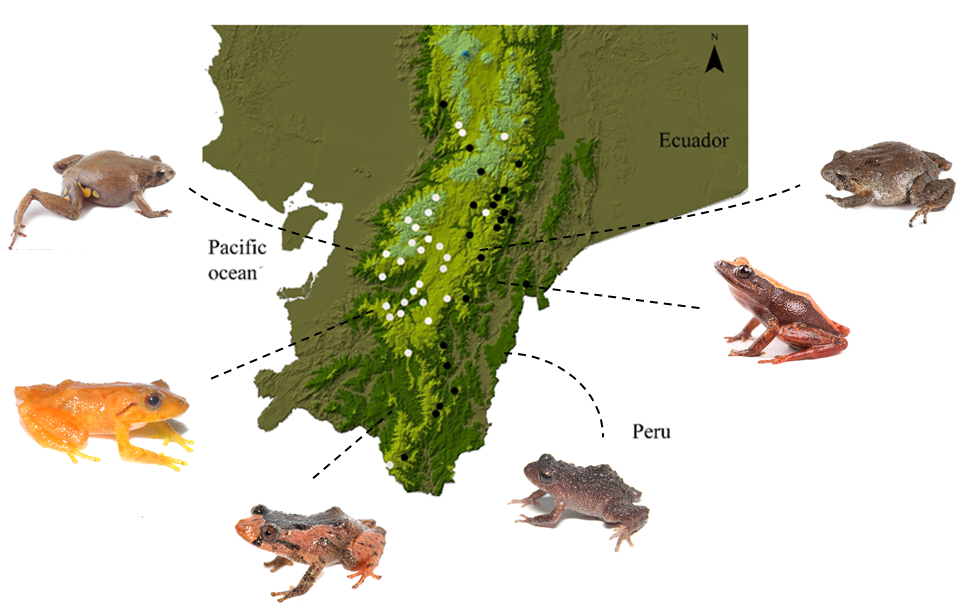
\includegraphics[width=13.71in]{figure1} 

}

\caption{Map of southern Ecuador, showing some representative members of the *P. orestes* group}\label{fig:plot1}
\end{figure}

\hypertarget{the-data}{%
\section{The data}\label{the-data}}

The data from this project includes the following:

\begin{enumerate}
\def\labelenumi{\arabic{enumi}.}
\tightlist
\item
  \textbf{Morphometric data} obtained from external structures measured to the neares 0.1mm. Acronyms follow Waters et al.~(2016)

  \begin{itemize}
  \tightlist
  \item
    eye to nostril distance (EN)
  \item
    head length (HL)
  \item
    head width (HW)
  \item
    interorbital distance (IOD)
  \item
    internarial distance (IND)
  \item
    snout vent length (SVL)
  \item
    tibia length (TL)
  \item
    foot length (FL)
  \item
    tympanum diameter (TD)
  \item
    eye diameter (ED)
  \item
    upper eyelid width (EW)
  \item
    Toe pad width (TDW)
  \item
    Finger pad width (FDW)
  \item
    HAND lenght (HANDL)
  \item
    Finger IV lenght (Finger.width)
  \end{itemize}
\item
  \textbf{Natural history data} for each recorded invidual obtained from direct observations in field, museum data bases and the map of continental ecosystems from the Ecuadorean environmental ministry.

  \begin{itemize}
  \tightlist
  \item
    Ecosystem
  \item
    microhabitat
  \item
    general observations regarding habitat conditions
  \end{itemize}
\item
  \textbf{Molecular data} from sanger sequencing of two mithocondrial and one nuclear genes

  \begin{itemize}
  \tightlist
  \item
    12S
  \item
    16H single fragment aligned reads
  \item
    16SC single fragment aligned
  \item
    Rag-1
  \item
    16S combined fragments
  \end{itemize}
\item
  \textbf{Geographical data} obtained from museum records, field journals from collectors or taken directly in the field with a GPS

  \begin{itemize}
  \tightlist
  \item
    locality
  \item
    coordinates x
  \item
    coordinates y
  \item
    elevation m
  \end{itemize}
\end{enumerate}

\hypertarget{data-base-structure}{%
\section{Data base structure}\label{data-base-structure}}

The data base structure for SQLite is based on 5 tables. The reference column in every table is the \emph{museum\_code}, which if formed by the acronyms of each museum collection followed by a 3 to 7 digits number.

\begin{figure}

{\centering 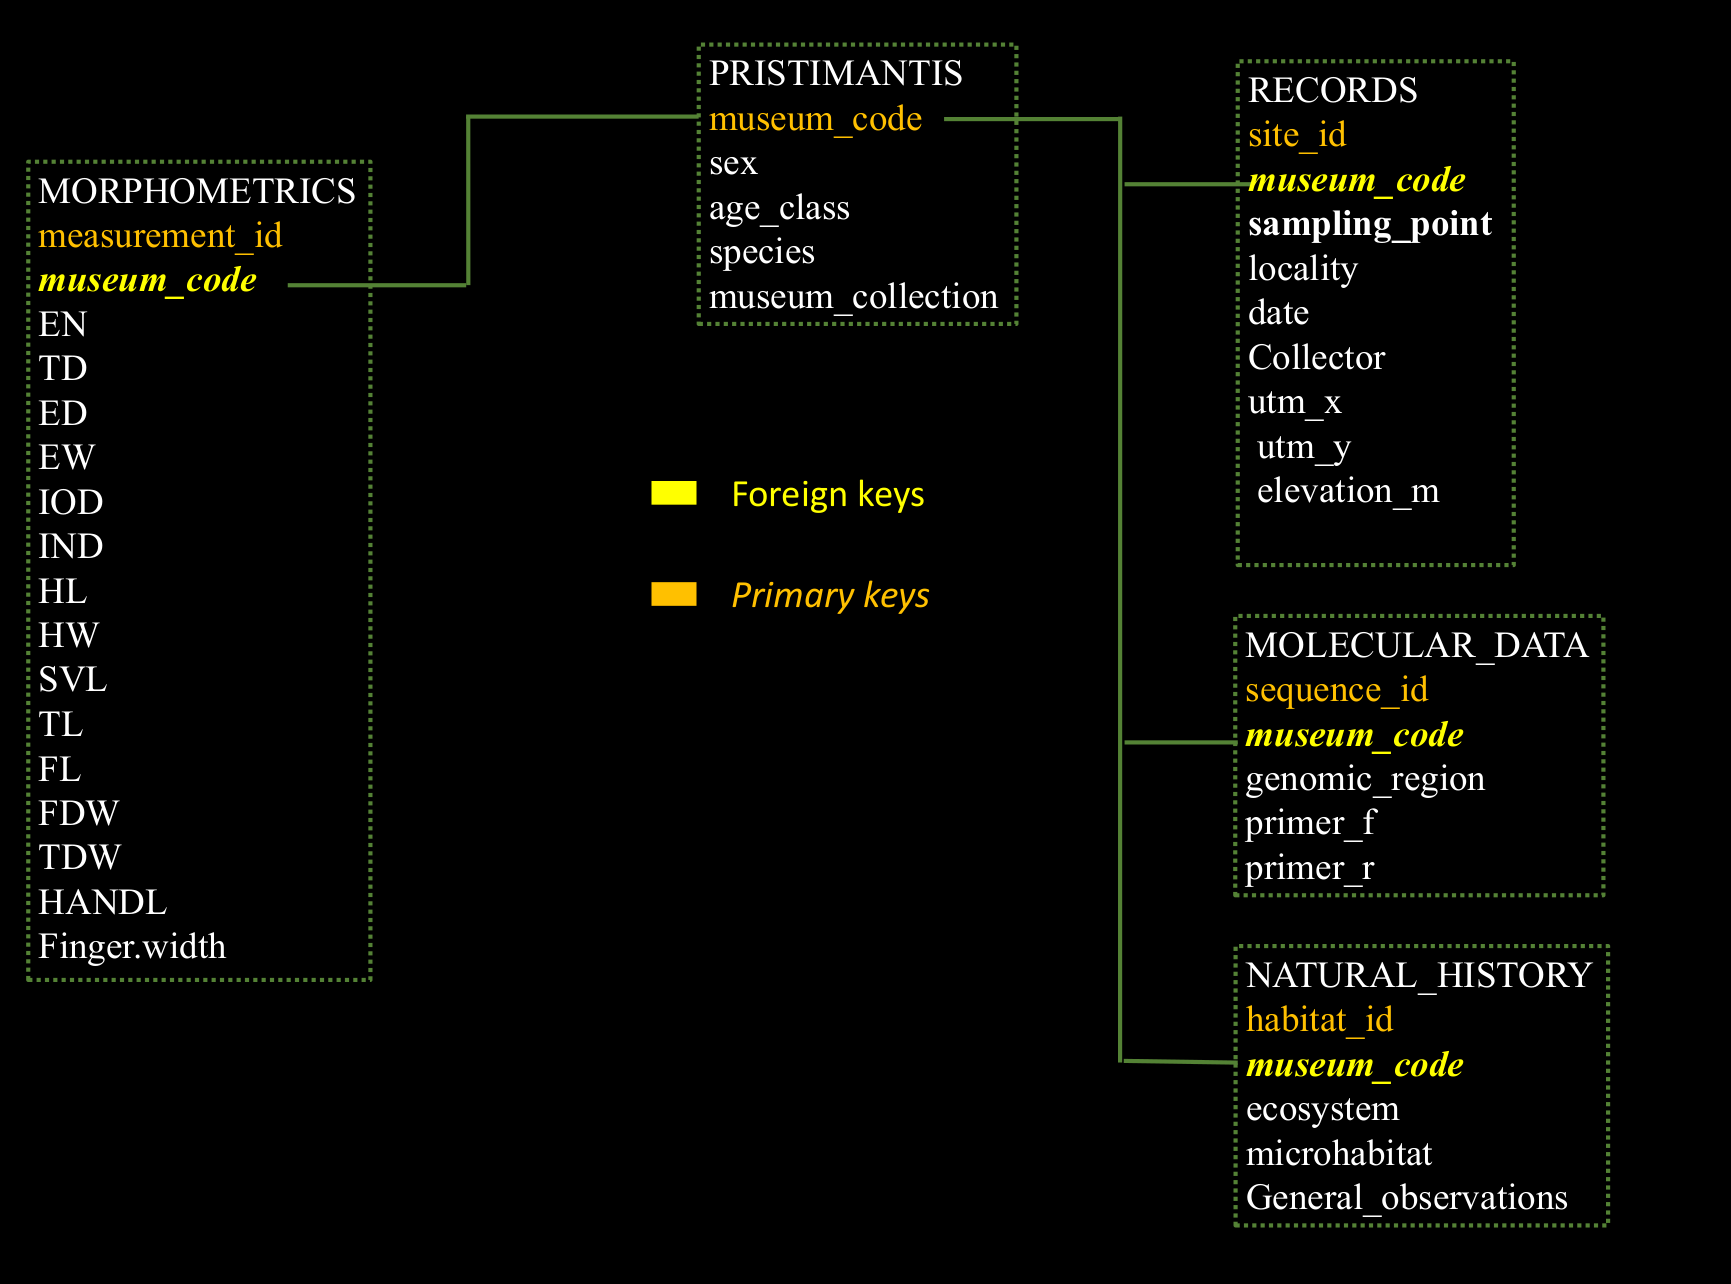
\includegraphics[width=21.64in,height=2\textheight]{figure2} 

}

\caption{Data base structure}\label{fig:plot2}
\end{figure}

Calling packages BDI and RSQLite

\begin{Shaded}
\begin{Highlighting}[]
\FunctionTok{library}\NormalTok{(DBI)}
\FunctionTok{library}\NormalTok{(RSQLite)}
\FunctionTok{library}\NormalTok{(tidyverse)}
\FunctionTok{library}\NormalTok{(viridis)}
\end{Highlighting}
\end{Shaded}

Creating orestes.db

\begin{Shaded}
\begin{Highlighting}[]
\NormalTok{orestes\_db }\OtherTok{\textless{}{-}} \FunctionTok{dbConnect}\NormalTok{(RSQLite}\SpecialCharTok{::}\FunctionTok{SQLite}\NormalTok{(), }\StringTok{"orestes.db"}\NormalTok{)}
\end{Highlighting}
\end{Shaded}

\hypertarget{table-1-general-information}{%
\subsection{Table 1 General information}\label{table-1-general-information}}

This table includes five rows and has general data from each collected invididual including the museum\_id, sex, age class, species name, and museum collection name.

\begin{Shaded}
\begin{Highlighting}[]
\FunctionTok{dbExecute}\NormalTok{(orestes\_db, }\StringTok{"CREATE TABLE pristimantis (}
\StringTok{museum\_id varchar(10) NOT NULL,}
\StringTok{sex char(3) CHECK (sex IN (\textquotesingle{}M\textquotesingle{}, \textquotesingle{}F\textquotesingle{}, \textquotesingle{}NA\textquotesingle{})),}
\StringTok{age\_class varchar(8) CHECK (age\_class IN (\textquotesingle{}Juvenile\textquotesingle{}, \textquotesingle{}Subadult\textquotesingle{}, \textquotesingle{}Adult\textquotesingle{}, \textquotesingle{}NA\textquotesingle{})),}
\StringTok{species varchar(50),}
\StringTok{museum\_collection varchar (10),}
\StringTok{PRIMARY KEY (museum\_id)}
\StringTok{);"}\NormalTok{)}
\end{Highlighting}
\end{Shaded}

Calling data from csv sheet

\begin{Shaded}
\begin{Highlighting}[]
\NormalTok{pristimantis }\OtherTok{\textless{}{-}} \FunctionTok{read.csv}\NormalTok{(}\StringTok{"1\_pristimantis.csv"}\NormalTok{, }\AttributeTok{fileEncoding=}\StringTok{"UTF{-}8{-}BOM"}\NormalTok{, }
                   \AttributeTok{stringsAsFactors =} \ConstantTok{FALSE}\NormalTok{) }

\FunctionTok{names}\NormalTok{(pristimantis)}
\end{Highlighting}
\end{Shaded}

\begin{verbatim}
## [1] "museum_id"         "sex"               "age_class"        
## [4] "species"           "museum_collection"
\end{verbatim}

Entering data into database

\begin{Shaded}
\begin{Highlighting}[]
\FunctionTok{dbWriteTable}\NormalTok{(orestes\_db, }\StringTok{"pristimantis"}\NormalTok{, pristimantis, }\AttributeTok{append =} \ConstantTok{TRUE}\NormalTok{)}

\FunctionTok{dbGetQuery}\NormalTok{(orestes\_db, }\StringTok{"SELECT * FROM pristimantis LIMIT 6;"}\NormalTok{)}
\end{Highlighting}
\end{Shaded}

\begin{verbatim}
##   museum_id  sex age_class                    species museum_collection
## 1   AES2208    F  Juvenile          Pristimantis sp19              MECN
## 2   AES2392    M  Juvenile          Pristimantis sp17              MECN
## 3   AES2450 <NA>      <NA> Pristimantis cf versicolor              MZUA
## 4   AES2451 <NA>      <NA>  Pristimantis bromeliaceus              MZUA
## 5   AES2457    F     Adult           Pristimantis sp2              MECN
## 6   AES2464 <NA>  Juvenile                       <NA>              MECN
\end{verbatim}

\hypertarget{table-2-records}{%
\subsection{Table 2 Records}\label{table-2-records}}

This table includes specific sampling point, locality name, province, date of collection, collectors name, geographic coordinates and elevation

\begin{Shaded}
\begin{Highlighting}[]
\FunctionTok{dbExecute}\NormalTok{(orestes\_db, }\StringTok{"CREATE TABLE records (}
\StringTok{record\_id INTEGER PRIMARY KEY AUTOINCREMENT,}
\StringTok{museum\_id varchar(10) NOT NULL,}
\StringTok{sampling\_point varchar (75),}
\StringTok{locality varchar (50),}
\StringTok{province varchar (20),}
\StringTok{date varchar (10),}
\StringTok{coordinates\_y double,}
\StringTok{coordinates\_x double,}
\StringTok{elevation double,}
\StringTok{collector varchar (150),}
\StringTok{FOREIGN KEY (museum\_id) REFERENCES pristimantis(museum\_id)}
\StringTok{);"}\NormalTok{)}
\end{Highlighting}
\end{Shaded}

Calling data from csv sheet

\begin{Shaded}
\begin{Highlighting}[]
\NormalTok{records }\OtherTok{\textless{}{-}} \FunctionTok{read.csv}\NormalTok{(}\StringTok{"2\_records\_new.csv"}\NormalTok{, }\AttributeTok{fileEncoding=}\StringTok{"UTF{-}8{-}BOM"}\NormalTok{, }
                   \AttributeTok{stringsAsFactors =} \ConstantTok{FALSE}\NormalTok{) }

\FunctionTok{names}\NormalTok{(records)}
\end{Highlighting}
\end{Shaded}

\begin{verbatim}
##  [1] "record_id"      "museum_id"      "sampling_point" "locality"      
##  [5] "province"       "date"           "coordinates_x"  "coordinates_y" 
##  [9] "elevation"      "collector"
\end{verbatim}

Entering data into database

\begin{Shaded}
\begin{Highlighting}[]
\FunctionTok{dbWriteTable}\NormalTok{(orestes\_db, }\StringTok{"records"}\NormalTok{, records, }\AttributeTok{append =} \ConstantTok{TRUE}\NormalTok{)}

\FunctionTok{dbGetQuery}\NormalTok{(orestes\_db, }\StringTok{"SELECT * FROM records LIMIT 6;"}\NormalTok{)}
\end{Highlighting}
\end{Shaded}

\begin{verbatim}
##   record_id museum_id   sampling_point   locality        province date
## 1         1   AES2208       Angas alto      Angas           Azuay <NA>
## 2         2   AES2392  Tinajillas alto Tinajillas Morona Santiago <NA>
## 3         3   AES2450 Tinajillas medio Tinajillas Morona Santiago <NA>
## 4         4   AES2451 Tinajillas medio Tinajillas Morona Santiago <NA>
## 5         5   AES2457 Tinajillas medio Tinajillas Morona Santiago <NA>
## 6         6   AES2464       Tinajillas Tinajillas Morona Santiago <NA>
##   coordinates_x coordinates_y elevation                        collector
## 1        689997       9679823      3949 Cristian Villalta, Ervin Ramirez
## 2        761408       9667836      3146 Cristian Villalta, Ervin Ramirez
## 3        768733       9666165      2195 Cristian Villalta, Ervin Ramirez
## 4        768733       9666165      2195 Cristian Villalta, Ervin Ramirez
## 5        768733       9666165      2195 Cristian Villalta, Ervin Ramirez
## 6        761408       9667836      3146 Cristian Villalta, Ervin Ramirez
\end{verbatim}

\hypertarget{table-3-molecular-data}{%
\subsection{Table 3 Molecular data}\label{table-3-molecular-data}}

This data table contains a sequence\_id, museum\_id, 12S base pairs, 16S base pairs, RAG-1 base pairs.

\begin{Shaded}
\begin{Highlighting}[]
\FunctionTok{dbExecute}\NormalTok{(orestes\_db, }\StringTok{"CREATE TABLE molecular\_dat (}
\StringTok{record\_id INTEGER PRIMARY KEY AUTOINCREMENT,}
\StringTok{museum\_id varchar(10) NOT NULL,}
\StringTok{gene\_12s integer,}
\StringTok{fragment\_16sc integer,}
\StringTok{fragment\_16h integer,}
\StringTok{gene\_RAG\_1 integer,}
\StringTok{FOREIGN KEY (museum\_id) REFERENCES pristimantis(museum\_id)}
\StringTok{);"}\NormalTok{)}
\end{Highlighting}
\end{Shaded}

Calling data from csv sheet

\begin{Shaded}
\begin{Highlighting}[]
\NormalTok{molecular }\OtherTok{\textless{}{-}} \FunctionTok{read.csv}\NormalTok{(}\StringTok{"3\_molecular\_data.csv"}\NormalTok{, }\AttributeTok{fileEncoding=}\StringTok{"UTF{-}8{-}BOM"}\NormalTok{, }
                   \AttributeTok{stringsAsFactors =} \ConstantTok{FALSE}\NormalTok{) }

\FunctionTok{names}\NormalTok{(molecular)}
\end{Highlighting}
\end{Shaded}

\begin{verbatim}
## [1] "record_id"     "museum_id"     "gene_12s"      "fragment_16sc"
## [5] "fragment_16h"  "gene_RAG_1"
\end{verbatim}

Entering data into database

\begin{Shaded}
\begin{Highlighting}[]
\FunctionTok{dbWriteTable}\NormalTok{(orestes\_db, }\StringTok{"molecular\_dat"}\NormalTok{, molecular, }\AttributeTok{append =} \ConstantTok{TRUE}\NormalTok{)}

\FunctionTok{dbGetQuery}\NormalTok{(orestes\_db, }\StringTok{"SELECT * FROM molecular LIMIT 6;"}\NormalTok{)}
\end{Highlighting}
\end{Shaded}

\begin{verbatim}
##   record_id museum_id X12s_bp X16s_bp RAG_1_bp
## 1         1   AES2475      NA     853       NA
## 2         2   AES2516     386     425       NA
## 3         3   AES2528      NA    1028      507
## 4         4   AES2539     585    1049       NA
## 5         5   AES2555      NA      NA       NA
## 6         6   AES2557     300    1002       NA
\end{verbatim}

\begin{figure}

{\centering 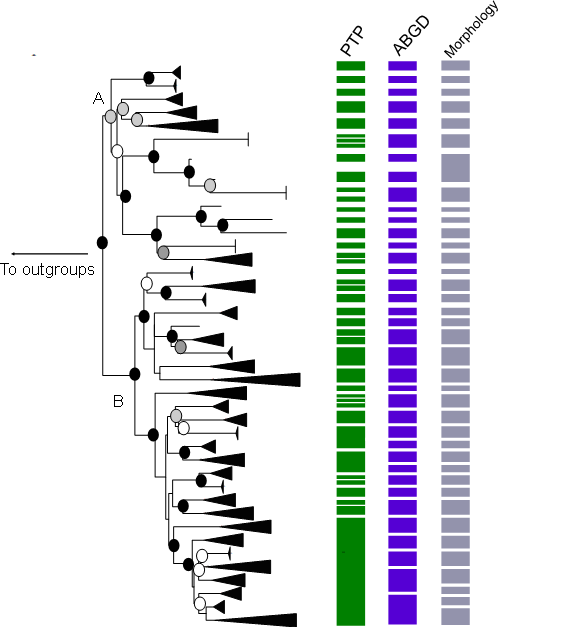
\includegraphics[width=7.01in,height=2\textheight]{figure3} 

}

\caption{Multigene phylogenetic tree of *Pristimantis orestes*}\label{fig:plot3}
\end{figure}

\hypertarget{table-4-natural-history}{%
\subsection{Table 4 Natural history}\label{table-4-natural-history}}

This data table contains information regarding the microhabitat and substrate were each individual was found.

\begin{Shaded}
\begin{Highlighting}[]
\FunctionTok{dbExecute}\NormalTok{(orestes\_db, }\StringTok{"CREATE TABLE habitat (}
\StringTok{habitat\_id INTEGER PRIMARY KEY AUTOINCREMENT,}
\StringTok{museum\_id varchar(10) NOT NULL,}
\StringTok{ecosystem varchar (50), }
\StringTok{microhabitat varchar (100), }
\StringTok{FOREIGN KEY (museum\_id) REFERENCES pristimantis(museum\_id)}
\StringTok{);"}\NormalTok{)}
\end{Highlighting}
\end{Shaded}

Calling data from csv sheet

\begin{Shaded}
\begin{Highlighting}[]
\NormalTok{habitat }\OtherTok{\textless{}{-}} \FunctionTok{read.csv}\NormalTok{(}\StringTok{"4\_habitat.csv"}\NormalTok{, }\AttributeTok{fileEncoding=}\StringTok{"UTF{-}8{-}BOM"}\NormalTok{, }
                   \AttributeTok{stringsAsFactors =} \ConstantTok{FALSE}\NormalTok{) }
\FunctionTok{names}\NormalTok{(habitat)}
\end{Highlighting}
\end{Shaded}

\begin{verbatim}
## [1] "habitat_id"   "museum_id"    "ecosystem"    "microhabitat"
\end{verbatim}

Entering data into database

\begin{Shaded}
\begin{Highlighting}[]
\FunctionTok{dbWriteTable}\NormalTok{(orestes\_db, }\StringTok{"habitat"}\NormalTok{, habitat, }\AttributeTok{append =} \ConstantTok{TRUE}\NormalTok{)}

\FunctionTok{dbGetQuery}\NormalTok{(orestes\_db, }\StringTok{"SELECT * FROM habitat LIMIT 6;"}\NormalTok{)}
\end{Highlighting}
\end{Shaded}

\begin{verbatim}
##   habitat_id museum_id
## 1         NA MECN12222
## 2         NA   MZUA726
## 3         NA  MZUA1926
## 4         NA QCAZ61156
## 5         NA QCAZ63665
## 6         NA QCAZ61152
##                                                                         ecosystem
## 1                                                             Herbazal del Páramo
## 2      Bosque siempreverde montano del Sur de la Cordillera Oriental de los Andes
## 3 Bosque siempreverde montano alto del Sur de la Cordillera Oriental de los Andes
## 4      Bosque siempreverde montano del Sur de la Cordillera Oriental de los Andes
## 5      Bosque siempreverde montano del Sur de la Cordillera Oriental de los Andes
## 6                            Bosque siempreverde montano alto del Catamayo-Alamor
##   microhabitat general_observations
## 1           NA                   NA
## 2           NA                   NA
## 3           NA                   NA
## 4           NA                   NA
## 5           NA                   NA
## 6           NA                   NA
\end{verbatim}

\hypertarget{table-5-morphometrics}{%
\subsection{Table 5 Morphometrics}\label{table-5-morphometrics}}

This data table contains morphometrics measurements from external characters. All measurements are rounded to the near 0.1mm and follow the definitions of Duelman \& Lehr (2009) and Watters et al.~(2016)

\begin{Shaded}
\begin{Highlighting}[]
\FunctionTok{dbExecute}\NormalTok{(orestes\_db, }\StringTok{"CREATE TABLE morphometrics (}
\StringTok{measurement\_id INTEGER PRIMARY KEY AUTOINCREMENT,}
\StringTok{EN\_mm float,}
\StringTok{TD\_mm float,}
\StringTok{ED\_mm float,}
\StringTok{EW\_mm float,}
\StringTok{IOD\_mm float,}
\StringTok{HL\_mm float,}
\StringTok{HW\_mm float,}
\StringTok{SVL\_mm float, }
\StringTok{TL\_mm float, }
\StringTok{FDW\_mm float,}
\StringTok{TDW\_mm float,}
\StringTok{HANDL\_mm float,}
\StringTok{finger.width\_mm,}
\StringTok{FOREIGN KEY (museum\_id) REFERENCES pristimantis(museum\_id)}
\StringTok{);"}\NormalTok{)}
\end{Highlighting}
\end{Shaded}

Calling data from csv sheet

\begin{Shaded}
\begin{Highlighting}[]
\NormalTok{morphometrics }\OtherTok{\textless{}{-}} \FunctionTok{read.csv}\NormalTok{(}\StringTok{"5\_morphometrics.csv"}\NormalTok{, }\AttributeTok{fileEncoding=}\StringTok{"UTF{-}8{-}BOM"}\NormalTok{, }
                   \AttributeTok{stringsAsFactors =} \ConstantTok{FALSE}\NormalTok{) }

\FunctionTok{names}\NormalTok{(morphometrics)}
\end{Highlighting}
\end{Shaded}

\begin{verbatim}
##  [1] "measurement_id"  "museum_id"       "EN_mm"           "TD_mm"          
##  [5] "ED_mm"           "EW_mm"           "IOD_mm"          "IND_mm"         
##  [9] "HL_mm"           "HW_mm"           "SVL_mm"          "TL_mm"          
## [13] "FL_mm"           "FDW_mm"          "TDW_mm"          "HANDL_mm"       
## [17] "Finger.width_mm"
\end{verbatim}

Entering data into database

\begin{Shaded}
\begin{Highlighting}[]
\FunctionTok{dbWriteTable}\NormalTok{(orestes\_db, }\StringTok{"morphometrics"}\NormalTok{, morphometrics, }\AttributeTok{append =} \ConstantTok{TRUE}\NormalTok{)}

\FunctionTok{dbGetQuery}\NormalTok{(orestes\_db, }\StringTok{"SELECT * FROM morphometrics LIMIT 6;"}\NormalTok{)}
\end{Highlighting}
\end{Shaded}

\begin{verbatim}
##   measurement_id museum_id EN_mm TD_mm ED_mm EW_mm IOD_mm IND_mm HL_mm HW_mm
## 1              1  MZUA1954  1.86  1.69  2.21  1.54   2.83   2.09  6.58  7.40
## 2              2 MECN10799  3.54  1.00  1.54  1.24   2.51   2.58  9.04  8.63
## 3              3 QCAZ45142  3.16  0.55  2.03  1.48   2.13   2.15  8.22  7.45
## 4              4 QCAZ45132  2.78  0.62  1.54  1.13   2.62   1.96  7.46  6.69
## 5              5 QCAZ45096  2.24  0.63  1.63  1.36   2.26   1.47  6.63  7.34
## 6              6 QCAZ46990  1.70  0.59  1.32  1.20   2.94   2.08   6.6  7.56
##   SVL_mm TL_mm FL_mm FDW_mm TDW_mm HANDL_mm Finger.width_mm
## 1  18.89  8.48  7.48   0.83   0.85     4.66            0.56
## 2  20.90 10.75  8.96   0.62   0.65       NA              NA
## 3  19.67  9.90  9.42   0.53   0.63       NA              NA
## 4  17.98  8.38  7.60   0.65   0.53       NA              NA
## 5  19.16  8.21  7.53   0.52   0.59       NA              NA
## 6  22.01  7.51  8.06   0.51   0.64       NA              NA
\end{verbatim}

\hypertarget{systematics-of-pristimantis-in-the-ecuadorean-andes}{%
\chapter{Systematics of Pristimantis in the ecuadorean Andes}\label{systematics-of-pristimantis-in-the-ecuadorean-andes}}

The phylogenetic analysis includes newly generated sequences from 199 individuals collected during field surveys. Figure 3.1 show the number of gene fragments amplified from the newly generated data. The final dataset included 222 genetically unique individuals, with a concatenated dataset of 2499 bp and included previously generated data from GenBank.

\begin{Shaded}
\begin{Highlighting}[]
\NormalTok{data1 }\OtherTok{\textless{}{-}}\NormalTok{ molecular\_data }\SpecialCharTok{\%\textgreater{}\%}  
  \FunctionTok{mutate}\NormalTok{(}\AttributeTok{gene\_16s =} \FunctionTok{ifelse}\NormalTok{(fragment\_16sc }\SpecialCharTok{\textgreater{}} \DecValTok{1} \SpecialCharTok{||}\NormalTok{ fragment\_16h }\SpecialCharTok{\textgreater{}} \DecValTok{1}\NormalTok{, }\DecValTok{1}\NormalTok{, }\DecValTok{0}\NormalTok{)) }\SpecialCharTok{\%\textgreater{}\%} 
  \FunctionTok{select}\NormalTok{(}\SpecialCharTok{{-}}\NormalTok{fragment\_16sc, }\SpecialCharTok{{-}}\NormalTok{fragment\_16h) }\SpecialCharTok{\%\textgreater{}\%} 
  \FunctionTok{pivot\_longer}\NormalTok{(}\AttributeTok{cols =} \FunctionTok{starts\_with}\NormalTok{(}\StringTok{"gene"}\NormalTok{),}
               \AttributeTok{names\_to =} \StringTok{"fragments"}\NormalTok{,}
               \AttributeTok{values\_to =} \StringTok{"bp"}\NormalTok{,}
               \AttributeTok{values\_drop\_na =} \ConstantTok{TRUE}\NormalTok{)}

\NormalTok{graph3}\FloatTok{.1} \OtherTok{\textless{}{-}} \FunctionTok{ggplot}\NormalTok{(}\AttributeTok{data =}\NormalTok{ data1, }\FunctionTok{aes}\NormalTok{(}\AttributeTok{x =}\NormalTok{ fragments, }\AttributeTok{fill =}\NormalTok{ fragments)) }\SpecialCharTok{+}
  \FunctionTok{geom\_bar}\NormalTok{(}\AttributeTok{stat =} \StringTok{"count"}\NormalTok{) }\SpecialCharTok{+}
  \FunctionTok{scale\_fill\_viridis}\NormalTok{(}\AttributeTok{discrete =}\NormalTok{ T) }\SpecialCharTok{+}
  \FunctionTok{theme\_classic}\NormalTok{() }\SpecialCharTok{+}
  \FunctionTok{labs}\NormalTok{(}\AttributeTok{x =} \StringTok{"Amplified Gene fragments"}\NormalTok{ , }\AttributeTok{y =} \StringTok{"Individuals"}\NormalTok{)}

\NormalTok{graph3}\FloatTok{.1}
\end{Highlighting}
\end{Shaded}


  \bibliography{book.bib,packages.bib}

\end{document}
